
\section{Interlude: A first look at polynomial equations} 

Nyx is making a blanket out of 3" $\times$ 3" squares of fabric in the middle and long strips of fabric for the border.  They have decided to make the blanket 7 squares longer than it is wide. So, for example, if they use 10 squares across, they will use $10+7=17$ squares down.  They will do a 4" border on the top and bottom of the blanket but only a 2.5" border on the left and right.

\begin{center}
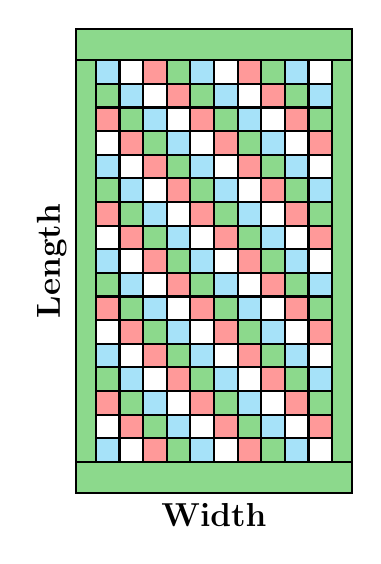
\begin{tikzpicture}[scale=0.1, line join=miter] % Adjust scale to fit your page size
    % Define custom colors
    \colorlet{babyblue}{cyan!35!white}
    \colorlet{quiltpink}{pink!80!red}
    \colorlet{sagegreen}{green!50!gray!60!white}

    % Fill interior squares with a 4-color repeating sequence (10x17 grid)
    \foreach \x in {0,3,...,27} {
        \foreach \y in {0,3,...,48} {
            % Calculate 4-cycle index based on grid positions
            \pgfmathparse{int(mod(\x/3 + \y/3, 4))}
            \ifcase\pgfmathresult
                \fill[babyblue] (\x,\y) rectangle (\x+3,\y+3);
            \or
                \fill[white] (\x,\y) rectangle (\x+3,\y+3);
            \or
                \fill[quiltpink] (\x,\y) rectangle (\x+3,\y+3);
            \or
                \fill[sagegreen] (\x,\y) rectangle (\x+3,\y+3);
            \fi
        }
    }

    % Fill sage green borders (Left/Right: 2.5", Top/Bttom: 4")
    \fill[sagegreen] (-2.5,0) rectangle (0,51);          % Left border
    \fill[sagegreen] (30,0) rectangle (32.5,51);         % Right border
    \fill[sagegreen] (-2.5,-4) rectangle (32.5,0);       % Bottom border
    \fill[sagegreen] (-2.5,51) rectangle (32.5,55);      % Top border

    % Draw grid lines over the filled squares
    \draw[thick, step=3cm] (0,0) grid (30,51);

    % Draw border outlines
    \draw[thick] (-2.5,0) rectangle (0,51);               % Left border
    \draw[thick] (30,0) rectangle (32.5,51);              % Right border
    \draw[thick] (-2.5,-4) rectangle (32.5,0);            % Bottom border
    \draw[thick] (-2.5,51) rectangle (32.5,55);           % Top border

    % Add labels
    \node[below, font=\large\bfseries] at (15, -4) {Width};
    \node[left, font=\large\bfseries, rotate=90, anchor=south] at (-2.5, 25.5) {Length};
\end{tikzpicture}
\end{center}

\subsection*{Different Sizes of Blanket}

What size blanket will Nyx make if they use 10 squares across, as shown in the picture?
The width of the blanket will include the left border (2.5"), the width of the 10 squares ($10 \times 3"$), and the right border (2.5"), so the blanket will be $$2.5+10\times3+2.5 = 35"
$$
wide.  Notice that we add the width of the border twice so instead of adding 2.5" twice, we can add $2 \times 2.5" = 5"$ once.  We can then simplify our calculation to $$10\times3+5 = 35"
$$
wide. 

The length of the blanket will include the top border (4"), the length of the $10+7=17$ squares ($(10+7) \times 3"$), and the right border (4"), so the blanket will be $$4+(10+7)\times 3+4 = 59"$$
long. As before, instead of adding 4" twice, we can add $2 \times 4"=8"$ once.  We can then simplify our calculation to $$(10+7)\times 3+8 = 59"$$ long.
The blanket will be $35" \times 59"$ which is a good size for a baby's crib.

Let's do a few more examples.  Let's underline the number of squares to help us see a pattern. If Nyx uses only 2 squares, then 
$$\text{width: }\underline{2}\times3+5 = 11"$$
and 
$$\text{length: }(\underline{2}+7)\times3+8 = 35"$$
The blanket will be $11" \times 35"$ which might be a good size for a doll.

If Nyx uses 20 squares, then
$$\text{width: }\underline{20}\times3+5 = 65"$$
and 
$$\text{length: }(\underline{20}+7)\times3+8 = 86"$$
The blanket will be $65" \times 86"$ which would fit a twin bed.

\subsection*{Linear models for blanket dimensions}

First, the variables are 
    $$S = \text{ number of squares (squares)} \sim \text{indep}$$
    $$W = \text{ width of blanket (inches)} \sim \text{dep}$$
    $$L = \text{ length of blanket (inches)} \sim \text{dep}$$

We can summarize our examples in a table.

\begin{center}
    \begin{tabular}{c|c|c|c}
        $S$ & 2 & 10 & 20 \\ \hline
        $W$ & 11 & 35 & 65 \\ \hline
        $L$ & 35 & 59 & 86
    \end{tabular}
\end{center}

When we graph both dependences, we see that the points fall on a line, so we have linear functions. 

\begin{center}
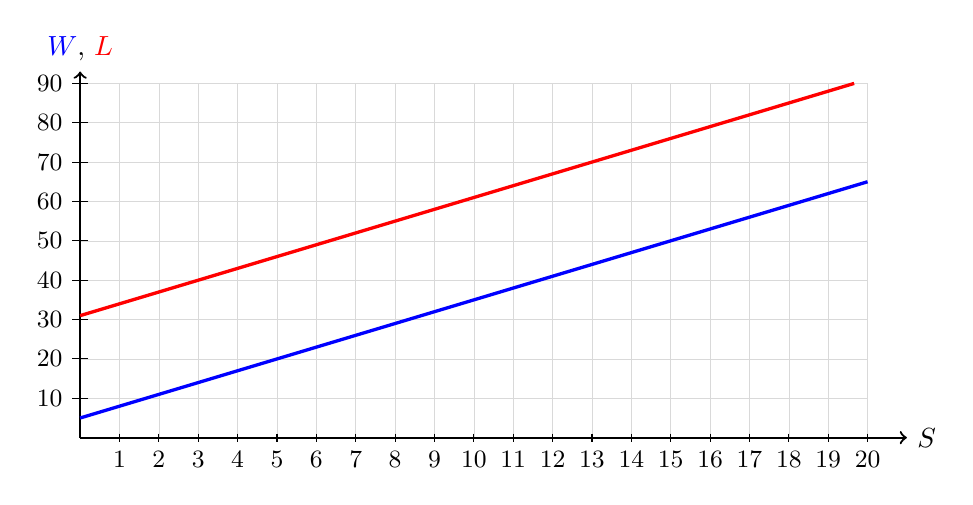
\begin{tikzpicture}[xscale=0.5, yscale=0.05]
    % Draw horizontal grid lines every 10 units along the vertical axis (up to 90)
    \foreach \y in {10,20,...,90} {
        \draw[gray!30, very thin] (0,\y) -- (20,\y);
    }

    % Draw vertical grid lines every 1 unit along S (up to 20)
    \foreach \x in {1,2,...,20} {
        \draw[gray!30, very thin] (\x,0) -- (\x,90);
    }

    % Draw axes with tick marks and labels
    \draw[thick, ->] (0,0) -- (21,0) node[right] {$S$};
    \draw[thick, ->] (0,0) -- (0,93) node[above] {{\color{blue}$W$}, {\color{red}$L$}};

    % X-axis tick marks every 1 up to 20
    \foreach \x in {1,2,...,20} {
        \draw (\x, 1) -- (\x, -1) node[below] {\small \x};
    }

    % Y-axis tick marks every 10 up to 90
    \foreach \y in {10,20,...,90} {
        \draw (0.2, \y) -- (-0.2, \y) node[left] {\small \y};
    }

    % Plot W = 3S + 5 in blue
    \draw[very thick, blue] plot[domain=0:20] (\x, {3*\x + 5});

    % Plot L = 3S + 31 in red
    \draw[very thick, red] plot[domain=0:19.66] (\x, {3*\x + 31});
\end{tikzpicture}
\end{center}

\subsection*{Equations for the width and length of blanket}

Let's write equations for the width and for the length of Nyx's blanket, each a function of the number of squares they use.

First, the width.  In our example, Nyx used $S=10$ squares across and the width of the blanket was
$$\underline{10} \times 3 + 5 = 35"$$
Our equation is $$\text{width: }S \times 3 + 5 = W.$$ Let's write the dependent variable on the left-hand side of the equation, and use algebraic notation to write $3S$ instead of $S \times 3$.  Our equation is then $$W = 3S + 5$$

Next, the length. In our example,  Nyx used $S=10$ squares across and the length of the blanket was $$(\underline{10}+7) \times 3+8 = 59".$$
Our equation is $$(S+7) \times 3+8 = L,$$ which we can rewrite as $$L = 3(S+7)+8.$$

\subsection*{The Distributive Property}

But, wait!  We could have calculated the length differently.  We can think of the length as having three parts: $3S$ which is the length of the $S$ squares, $3 \times 7 = 21$ which is the length of the additional 7 squares, and $2 \times 4 = 8$ which is the length of the top and bottom borders.  Breaking into these pieces we get a new equation for the length:
$$L = 3S + 21 + 8$$
which can be simplified further to 
$$L = 3S + 29$$

Does this new equation make sense?  The 3"/square represents the length of each square Nyx uses.  The 29" is the part of the length of the 7 squares and top/bottom borders combined.  Okay.

Uh oh! That means we have two different looking equations for the length
$$L = 3(S+7)+8 \text{ and }
L=3S + 29.$$
There must be some reason why these equations are actually the same. 

The distributive property is the secret.  It says that 
 $$3(S+7)=3 \times (S+7) = (3 \times S) + (3 \times 7) = 3S + 21.$$  
 Here's a picture illustrating the distributive property.

 \begin{center}
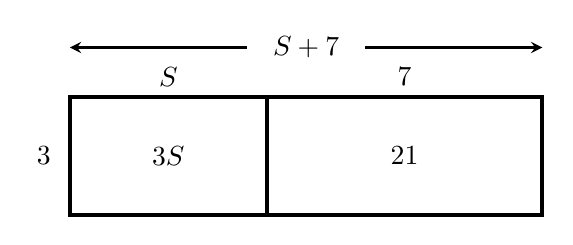
\begin{tikzpicture}[line width=1.5pt, scale = .5]
    % Main Rectangle (S=5 units wide + 7 units wide = 12 total, 3 tall)
    \draw (0,0) rectangle (12,3);
    % Vertical Divider at S=5 units from left
    \draw (5,0) -- (5,3);
    % Top Label and arrows
    \draw[<-, >=stealth, line width=0.8pt] (0, 4.25) -- (4.5, 4.25);
    \node at (6, 4.25) {$S+7$};
    \draw[->, >=stealth, line width=0.8pt] (7.5, 4.25) -- (12, 4.25);
    % Sub-top labels
    \node at (2.5, 3.5) {$S$};
    \node at (8.5, 3.5) {$7$};
    % Left Label
    \node[left] at (-0.2, 1.5) {$3$};
    % Inner labels
    \node at (2.5, 1.5) {$3S$};
    \node at (8.5, 1.5) {$21$};

\end{tikzpicture}
 \end{center}
 
Going back we can use the distributive property to write $$L = 3(S+7) + 10 = 3S +21 + 8 = 3S + 29$$
which is exactly the other version of the equation.  Whew.   

\subsection*{Area of Blanket}

Nyx has decided after they finish the blanket, they will make it the top layer of a light comforter.  For that, Nyx will use plain fabric for the bottom layer and use some fiberfill to get a thickness of 2 inches in between. How much fiberfill do they need? 

To start, Nyx needs to know the area of the blanket. The area is the length times the width.  For the baby blanket that was 10 squares across, the width was 35" and the length was 59" so the area was $35 \times 59 = 2065$ square inches.  

We can write an equation for the area of the blanket using the variables
$$S = \text{ number of squares (squares) } \sim \text{indep}$$
$$A = \text{ area of blanket (square inches)} \sim \text{ dep}$$
We know that the area is the length times the width, so putting in our formulas we get 
$$A = (3S+29)(3S+5)$$

\subsection*{The FOIL property}

We can simplify the equation for area using the distributive property.  
\begin{eqnarray*}
    A &=& (3S+29)(3S+5) \\
    &=& (3S)(3S+5) + (29)(3S+5) \\
    &=& \underbrace{(3S)(3S)}_{\text{First}} + \underbrace{(3S)(5)}_{\text{Outside}}  + \underbrace{(29)(3S)}_{\text{Inside}} + \underbrace{(29)(5)}_{\text{Last}} \\
\end{eqnarray*}

Let's simplify each term separately.  The first product is 
$$(3S)(3S) = (3 \times 3)(S \times S) = 9S^2$$
The outside product is 
$$(3S)(5) = (3 \times 5)S = 15S$$
The inside product is 
$$(29)(3S) = (29 \times 3)S = 87S$$
And the last product is
$$(29)(5) = 29 \times 5 = 145$$
Maybe you've heard of FOIL?  That's short for First-Outside-Inside-Last which can help you remember how this multiplying out works.

Adding everything up and combining the like terms we get
$$A = 9S^2 + 15S + 87S + 145 = 9S^2 + (15+87)S + 145 = 9S^2+102S + 145$$

Here's a picture illustrating the FOIL property.

 \begin{center}
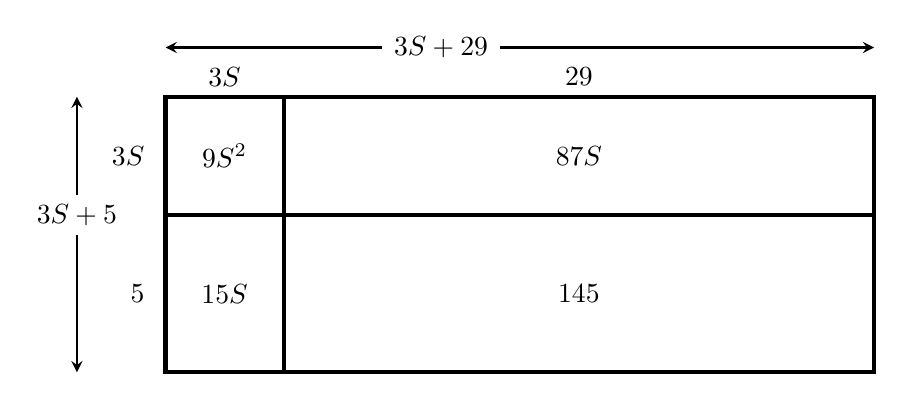
\begin{tikzpicture}[line width=1.5pt, scale =.5]
    % Main Rectangle 18 wide and 7 tall
    \draw (0,0) rectangle (18,7);
    % Vertical Divider at 3 units from left
    \draw (3,0) -- (3,7);
    % Horizontal Divider at 3 units from top = 4 units from bottom
    \draw (0,4) -- (18,4);
    % Top Label and arrows
    \draw[<-, >=stealth, line width=0.8pt] (0, 8.25) -- (5.5, 8.25);
    \node at (7, 8.25) {$3S+29$};
    \draw[->, >=stealth, line width=0.8pt] (8.5, 8.25) -- (18, 8.25);
    % Sub-top labels
    \node at (1.5, 7.5) {$3S$};
    \node at (10.5, 7.5) {$29$};
    % Left Label and arrow
    \draw[<-, >=stealth, line width=0.8pt] (-2.25, 0) -- (-2.25, 3.5);
    \node at (-2.25, 4) {$3S+5$};
    \draw[->, >=stealth, line width=0.8pt] (-2.25, 4.5) -- (-2.25, 7);
    % Sub-left labels
    \node[left] at (-0.25, 5.5) {$3S$};
    \node[left] at (-0.25, 2) {$5$};
    % Inner labels 
    \node at (1.5, 5.5) {$9S^2$};
    \node at (1.5, 2) {$15S$};
    \node at (10.5, 5.5) {$87S$};
    \node at (10.5, 2) {$145$};
\end{tikzpicture}
 \end{center}

That was a lot of algebra.  Here's a quicker version of what we just did so you can see it all in one place.
\begin{eqnarray*}
    A &=& (3S+29)(3S+5) \\
    &=& \underbrace{(3S)(3S)}_{\text{First}} + \underbrace{(3S)(5)}_{\text{Outside}}  + \underbrace{(29)(3S)}_{\text{Inside}} + \underbrace{(29)(5)}_{\text{Last}} \\
    &=& 9S^2+15S + 87S + 145 \\
    &=& 9S^2+102S + 145
\end{eqnarray*}

Let's double check, when $S=10$ we get
$$A = 9\times 10^2 + 102 \times 10 + 145 = 2065$$ as before.

\subsection*{A quadratic model}

As before, we make make a table and graph.  Using the same values for $S$ as before we get

\begin{center}
    \begin{tabular}{c|c|c|c}
        $S$ & 2 & 10 & 20 \\ \hline
        $A$ & 385 & 2065 & 5785
    \end{tabular}
\end{center}

\begin{center}
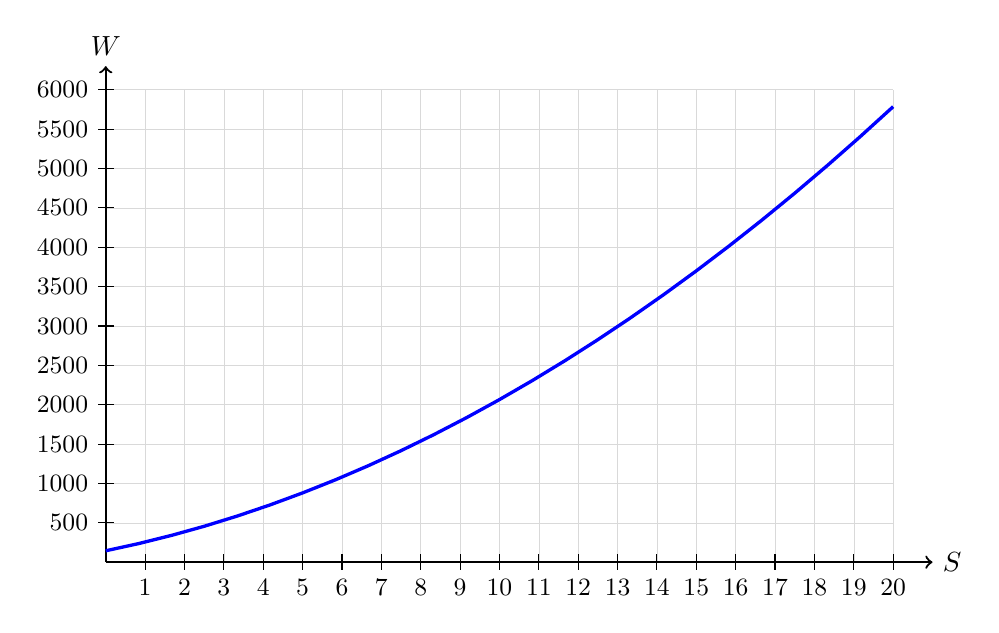
\begin{tikzpicture}[xscale=0.5, yscale=1]
    % Draw horizontal grid lines every 0.5 units (representing 500 up to 6000)
    \foreach \y in {0.5,1.0,...,6.0} {
        \draw[gray!30, very thin] (0,\y) -- (20,\y);
    }
    % Draw vertical grid lines every 1 unit along S (up to 20)
    \foreach \x in {1,2,...,20} {
        \draw[gray!30, very thin] (\x,0) -- (\x,6);
    }
    % Draw axes with tick marks and labels
    \draw[thick, ->] (0,0) -- (21,0) node[right] {$S$};
    \draw[thick, ->] (0,0) -- (0,6.3) node[above] {$W$};

    % X-axis tick marks every 1 up to 20
    \foreach \x in {1,2,...,20} {
        \draw (\x, 0.1) -- (\x, -0.1) node[below] {\small \x};
    }
    % Y-axis tick marks labeled in thousands (500 to 6000)
    \foreach \y/\label in {0.5/500, 1/1000, 1.5/1500, 2/2000, 2.5/2500, 3/3000, 3.5/3500, 4/4000, 4.5/4500, 5/5000, 5.5/5500, 6/6000} {
        \draw (0.2, \y) -- (-0.2, \y) node[left] {\small \label};
    }

    % Plot parabola dividing expression by 1000 to match scale
    \draw[very thick, blue] plot[domain=0:20] (\x, {(9*\x*\x + 102*\x + 145)/1000});
\end{tikzpicture}
\end{center}

We can see that the function is not linear because the graph is not a line.

\subsection*{Fiberfill}

To get a fluffy feel without being too heavy, Nyx has decided to use a premium cluster fiberfill to get 2" thick.  (Nyx will stitch the fill along every fabric join and at intervals along the border, in case you were wondering, because nobody likes a lumpy blanket.)  The clerk at the fabric store said that Nyx will need 14 ounces of fiberfill for 
every 1000 square inches of area.  Notice that $$\frac{14 \text{ ounces}}{1000 \text{ square inches}} = 0.14 \text{ ounces per square inch}$$
For example, for a baby quilt that's $35" \times 59"$, Nyx will need $0.14$ times the area.  That is, they will need $$0.14 \times2065 = 289.1$$ ounces of fiberfill.

We can write an equation for the amount of fiberfill as a function of the number of squares using 
    $$S = \text{ number of squares (squares)} \sim \text{indep}$$
    $$F = \text{ weight of fiberfill (ounces)} \sim \text{dep}$$

The equation is $$F = 0.14 (3S + 29)(3S + 5) = 0.14(9S2 + 102S + 145) = 1.26S^2 + 14.28S + 20.3$$
in case you were curious.

\subsection*{Another quadratic model}

Let's make a table and a graph for the fiberfill. First, we have 

\begin{center}
    \begin{tabular}{c|c|c|c}
        $S$ & 2 & 10 & 20 \\ \hline
        $F$ & 53.9 & 289.1 & 822.5
    \end{tabular}
\end{center}

\begin{center}
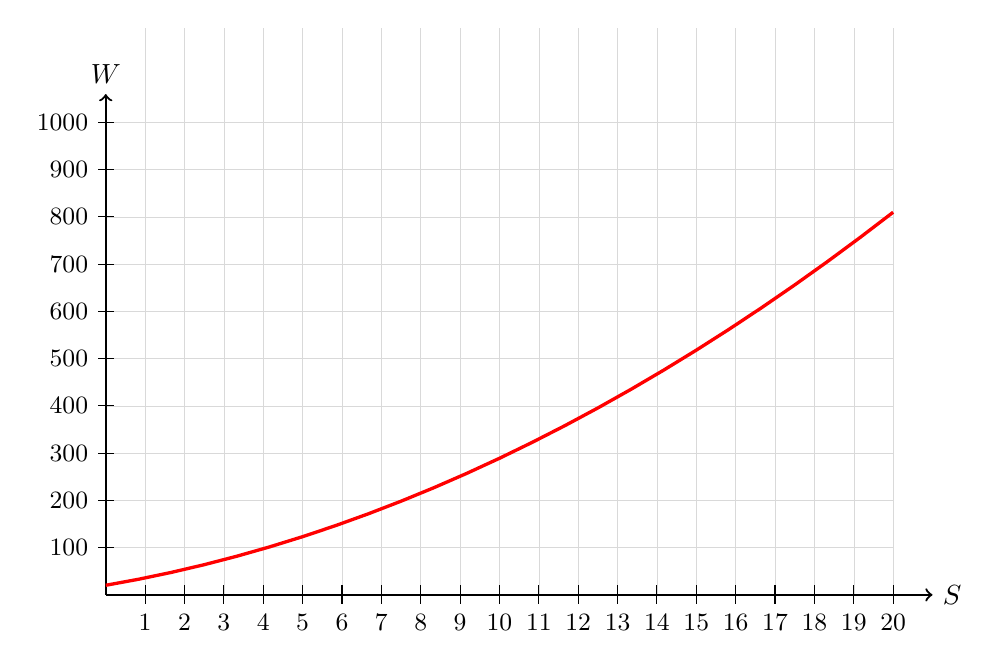
\begin{tikzpicture}[xscale=0.5, yscale=1.2]
    % Draw horizontal grid lines 
    \foreach \y in {0.5,1.0,...,5.0} {
        \draw[gray!30, very thin] (0,\y) -- (20,\y);
    }
    % Draw vertical grid lines every 
    \foreach \x in {1,2,...,20} {
        \draw[gray!30, very thin] (\x,0) -- (\x,6);
    }
    % Draw axes with tick marks and labels
    \draw[thick, ->] (0,0) -- (21,0) node[right] {$S$};
    \draw[thick, ->] (0,0) -- (0,5.3) node[above] {$W$};

    % X-axis tick marks
    \foreach \x in {1,2,...,20} {
        \draw (\x, 0.1) -- (\x, -0.1) node[below] {\small \x};
    }
    % Y-axis tick marks 
    \foreach \y/\label in {0.5/100, 1/200, 1.5/300, 2/400, 2.5/500, 3/600, 3.5/700, 4/800, 4.5/900, 5/1000} {
        \draw (0.2, \y) -- (-0.2, \y) node[left] {\small \label};
    }

    % Plot parabola dividing expression by 1000 to match scale
    \draw[very thick, red] plot[domain=0:20] (\x, {0.14*(9*\x*\x + 102*\x + 145)/200});
\end{tikzpicture}
\end{center}


\subsection*{Polynomial Equations}

Our equations for length and width were linear equations

$$W=3S+5$$
$$L=3(S+7)+8 \text{ or } L = 3S + 29$$

because they fit the standard linear equation template:  
$$ \text{dep } = \text{ start } + \text{ slope } * \text{ indep}$$

Our equations for the area and fiberfill were quadratic equations

$$A=(3S+31)(3S+5)\text{\quad or \quad}
A = 9S^2+108S + 155$$
$$F = 0.14 (3S + 29)(3S + 5) \text{\quad or \quad} F= 1.26S^2 + 14.28S + 20.3$$

because they fit the standard quadratic equation template: 
    $$\text{dep } = a*\text{indep}^2+b*\text{indep}+c$$

All of these equations are examples of  \textbf{polynomial equation}, meaning they can be written as the sum of multiples of powers of the independent variable.

\input{GoDoWS}

\noindent \textbf{Do you know \ldots}

\begin{itemize}
\item How to use geometry to find and area?
\item When to use the distributive property?
\item What FOIL stands for and how to multiply out expressions in parentheses?
 \input{NotSure} 
\end{itemize}

\subsection*{Exercises}

\begin{enumerate} 
%% WORKBOOK

\item Urban community gardens are catching on.  What was once an abandoned lot down the block is now a thriving 10'$\times$25' vegetable and berry garden for the neighborhood. (Remember ' stands for ``feet,'' so the garden is 10 feet wide and 25 feet long.)  One neighbor volunteered to donate gravel to make a path around the garden.  The path will be 3 inches deep and the same width all around. 

 \begin{center}
 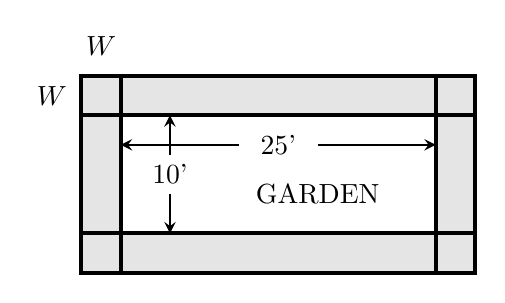
\begin{tikzpicture}[line width=1.5pt, scale=.5]
  % 1. Shaded Rectangles (Light Gray)
  % 4 Corner Rectangles
  \fill[gray!20] (0,0) rectangle (1,1);
  \fill[gray!20] (9,0) rectangle (10,1);
  \fill[gray!20] (0,4) rectangle (1,5);
  \fill[gray!20] (9,4) rectangle (10,5);

  % 4 Edge Rectangles
  \fill[gray!20] (1,0) rectangle (9,1);   % Bottom path
  \fill[gray!20] (1,4) rectangle (9,5);   % Top path
  \fill[gray!20] (0,1) rectangle (1,4);   % Left path
  \fill[gray!20] (9,1) rectangle (10,4);  % Right path

  % 2. Outer and Inner Outlines
  \draw (0,0) rectangle (10,5); % Outer Rectangle
  \draw (1,1) rectangle (9,4);  % Inner Garden Rectangle

  % 3. Individual Rectangle Outlines (Dividers between path sections)
  \draw (1,0) -- (1,1);
  \draw (9,0) -- (9,1);
  \draw (1,4) -- (1,5);
  \draw (9,4) -- (9,5);
  \draw (0,1) -- (1,1);
  \draw (0,4) -- (1,4);
  \draw (9,1) -- (10,1);
  \draw (9,4) -- (10,4);

  % 4. Labels
  % Label width of path in upper left corner
  \node at (-.75, 4.5) {$W$};
  \node at (0.5, 5.75) {$W$};

  % Label inside garden length
  \draw [<-, >=stealth, line width=0.8pt] (1, 3.25) -- (4, 3.25);
  \node at (5, 3.25) {25'};
  \draw [->, >=stealth, line width=0.8pt] (6, 3.25) -- (9, 3.25);

  % Label inside garden width
  \draw [<-, >=stealth, line width=0.8pt] (2.25, 1) -- (2.25, 2);
  \node at (2.25, 2.5) {10'};
  \draw [->, >=stealth, line width=0.8pt] (2.25, 3) -- (2.25, 4);
  % Add word Garden
  \node at (6, 2) {GARDEN};
\end{tikzpicture}
 \end{center}
 \hfill \emph{Story also appears in 2.3 Exercises 2.4 Exercises and 3.5 \#4}
\begin{enumerate}
\item The other measurements are in feet, so convert the depth of the path (3 inches) into feet also.  
\item Suppose for the moment that the path will be 4 feet wide. Calculate the area of the path.  Here's one way to do it:  first, find the area of the outer rectangle, then subtract the area of the garden itself.

\emph{Hint:  the length of that outer rectangle includes the 25 feet of garden plus the width of the path on each side.   Same for the width of that outer rectangle.}
\item Figure out how much gravel they would need (in cubic feet) for a 4 foot wide path by multiplying your answers to (a) and (b). 
\item  Actually, they aren't sure how wide the path should be and how much gravel they can get.  Let's write $W$ = width of path (feet).  Explain why the width of the outer rectangle is $10+2W$ and the length of the outer rectangle is $25+2W$.
\item Explain why the area of the path is $(10+2W)(25+2W)-250$.
\item Let's write $G$ = amount of gravel (cubic feet).  Write an equation for $G$ as a function of $W$.  Hint:  multiply your answers to (a) and (e).
\item Use FOIL and collecting like terms to simplify your answer to (f).  It should fit the quadratic equation template.  
\item Notice that if $W=0$, then $G=0$.  Explain what that means in terms of the story.
\end{enumerate}

\item Emery is selling custom printed laptop and water bottle sticker packs.  He is trying to understand how the number of sticker packs people will buy depends on the price.  There's a fancy name for the number of things people will buy -- it's called the \textbf{demand}. Emery knows from experience that if he prices sticker packs at \$10, then the demand is 200 sticker packs, but that the demand drops by 15 sticker packs per dollar increase in price. He identifies the variables
$$P = \text{ price of sticker packs (\$) } \sim \text{ indep}$$
$$D = \text{ demand (sticker packs) } \sim \text{ dep}$$

\begin{enumerate}
    \item How many sticker packs will Emery sell if he sets the price at \$11?  \$12? \$13?
    \item Make a table showing how demand depends on price, including $P= 10, 11, 12, 13$.
    \item Explain why the increase in price is calculated as $P-10$.
    \item Write an equation for the demand in terms of price.  Hint: Your equation will involve $(P-10)$.
    \item Use the distributive property and collect like terms to simplify your equation.  Hint: it is linear.
    \item Check that your simplified equation gives $D = 200$ when $P = 10$.
    \item What does your equation say the demand will be when $P=0$?  This answer does not make sense in the story.
    \item Draw a graph illustrating how the demand depends on the price.  Be sure to start at \$0.
    \begin{center}
\scalebox {.8} {
\includegraphics [width = 6in] {Graphics/GraphPaper.jpg}}
\end{center}
\end{enumerate}

\item In the previous problem, Emery was selling sticker packs.  Using the variables $$P = \text{ price of a sticker pack (\$) } \sim \text{ indep}$$
$$D = \text{ demand (sticker packs) } \sim \text{ dep}$$
Emery calculated that (spoiler alert) 
$$D = 350-15P$$
Notice that the intercept (price \$0) of 350 things doesn't really make any sense in the problem. Emery wants to figure out a price for sticker packs so that he can take in as much money as possible. There's a fancy name for that too -- the total amount of money Emery takes in is called the \textbf{total revenue}.  
\begin{enumerate}
    \item What is the total revenue if Emery prices sticker packs at \$10 and sells 200 of them?
    % Answer \$2000
    \item Make a table showing how revenue depends on price, including $P= 10, 11, 12, 13$.  Hint: use your answers for demand from the previous problem.
    \item Write an equation for the revenue in terms of price, using $$R = \text{ total revenue (\$) } \sim \text{ dep}$$  Hint: use your final equation from the previous problem.
    \item Use the distributive property and collect like terms to simplify your equation. Hint: it is quadratic.
    \item Check that your simplified equation gives $R = 2000$ when $P = 10$.
    \item What does your equation say the revenue will be when $P=0$ and what does that mean in the story?
    \item Draw a graph illustrating how the demand depends on the price.  Be sure to start at \$0.
    \begin{center}
\scalebox {.8} {
\includegraphics [width = 6in] {Graphics/GraphPaper.jpg}}
\end{center}
    \end{enumerate}

\item Ximena is trying to get some homework done so she wants to create a custom 24 ounce energy drink that has some caffeine, but not too much.  She has two available drinks that she can mix.

\begin{itemize}
    \item Rehab Monster: Green Tea\footnote{Source: \url{https://www.monsterenergy.com/en-us/energy-drinks/rehab-monster/green-tea/}} (10.3 mg caffeine/ounce)
    \item Snapple Peach Tea \footnote{Source: \url{https://snapple.com/products/snapple-peach-tea?filter=tea}} (2.3 mg caffeine/ounce)
\end{itemize}

She is interested in the variables 
$$M = \text{ amount of Rehab Monster (ounces) }\sim \text{indep}$$
$$C = \text{ amount of caffeine (mg)} \sim \text{ dep}$$

\begin{enumerate}
    \item If Ximena uses 10 ounces of Rehab Monster, how many ounces of Snapple Peach Tea will she use (remember she wants 24 ounces) and how much caffeine will that mixture have? %Answer 24-10 = 14, C = 10*10.3+14*2.3= 135.2 mg
    \item If she uses 16 ounces of Rehab Monster, how many ounces of Snapple Peach Tea will she use and how much caffeine with that mixture have?
    \item Write an equation describing how the total caffeine is a function of the amount of Rehab Monster.  Hint: How can we write the amount of Snapple Peach Tea in terms of $M$?
    \item Use the distributive property to simplify your equation.
\end{enumerate}

%% HOMEWORK 

\item Roy is mounting a $69'' \times 48''$ rectangular canvas painting on an aluminum composite panel. The panel covers the entire back of the painting and sticks out width $W$ inches around all four sides of the canvas. 

\begin{center}
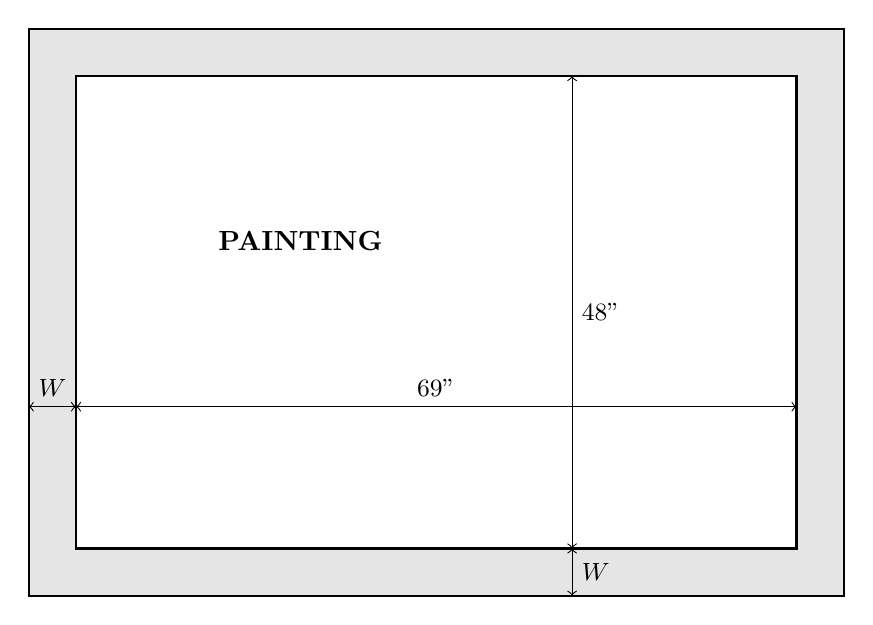
\begin{tikzpicture}[scale=0.15]
    % Outer Frame
    \draw[thick, fill=gray!20] (0,0) rectangle (69,48);
    % Inner Canvas
    \draw[thick, fill=white] (4,4) rectangle (65,44);
    % Labels
    \node at (23,30) {\textbf{PAINTING} };
    % Width arrows/labels
    \draw[<->] (0,16) -- (4,16) node[midway,above] {\small $W$};
    \draw[<->] (46,0) -- (46,4) node[midway,right] {\small $W$};
    \draw[<->] (4,16) -- (65,16) node[midway,above] {\small 69"};
    \draw[<->] (46,4) -- (46,44) node[midway,right] {\small 48"};
\end{tikzpicture}
\end{center}

\begin{enumerate}
    \item Suppose for the moment that the frame creates a border 3 inches wide ($W = 3$). Calculate the area of the aluminum panel. Note: the area is the area of the outside square, not just the border.
    \item Roy has not decided yet how wide the frame border should be. Let's write $W = \text{width of the frame border (inches)}$. Explain why the width of the outer frame is $69 + 2W$ and the length of the outer frame is $48 + 2W$.   
    \item Explain why the area of the aluminum panel is $(69 + 2W)(48 + 2W) $.
    
    \item Use FOIL and collecting like terms to simplify your answer to (c). It should fit the quadratic equation template.
    
    \item What is the area if $W=0$?  Explain what that means in terms of the story.
\end{enumerate}

\item Viviana is selling bottled cold brew coffee at a local weekend market. She is trying to understand how the number of bottles people will buy depends on the price per bottle. Viviana knows from experience that if she prices cold brew at \$4.00 per bottle, the demand is 150 bottles, but for every \$1 increase in price, the demand drops by 20 bottles. She writes the variables:
\begin{align*}
P &= \text{price of a cold brew bottle (\$) } \sim \text{indep} \\
D &= \text{demand (bottles) } \sim \text{dep}
\end{align*}

\begin{enumerate}
    \item How many bottles will Viviana sell if she sets the price at \$4.50? \$5.00? \$5.50?
    \item Make a table showing how demand depends on price, including $P = 4.00, 4.50, 5.00, 5.50$.
    \item Explain what $P-4$ represents in the story.
    \item Write an equation for demand in terms of price. Hint: Your equation will involve subtracting the demand drop from 150.
    \item Use the distributive property and collect like terms to simplify your equation. Hint: it is linear.
    \item Check that your simplified equation gives $D = 150$ when $P = 4$.
\end{enumerate}

\item In the previous problem, Viviana was selling bottled cold brew coffee. Using the variables:
\begin{align*}
P &= \text{price of a cold brew bottle (\$) } \sim \text{indep} \\
D &= \text{demand (bottles) } \sim \text{dep}
\end{align*}
she wrote an equation showing how the demand depends on the price.

Viviana wants to figure out a price for cold brew so that she can take in as much money total revenue as possible.

\begin{enumerate}
    \item What is the total revenue if Viviana prices cold brew at \$4.00 and sells 150 bottles?
    \item Make a table showing how revenue depends on price, including
    $P = 4.00, 4.50, 5.00, 5.50$. 
    Hint: use your answers for demand from the previous problem.
    \item Write an equation for the revenue in terms of price, using 
    $R = \text{total revenue (\$) } \sim \text{dep}$. 
    Hint: use your final equation for demand $D$ from the previous problem and the fact that
    $\text{Revenue} = \text{Price} \times \text{Demand}$.
    \item Use the distributive property to simplify your equation. Hint: it is quadratic.
    \item Check that your simplified equation gives $R = 600$ when $P = 4$.
\end{enumerate}

\item Kv\v{e}ta is working in a botany lab and needs to prepare a 30-gallon batch of liquid nutrient solution for a greenhouse experiment. She has two brands of concentrates available to mix:
\begin{itemize}
    \item \textbf{Hofner's:} contains 12 grams of nitrogen per gallon.
    \item \textbf{DeBoer's:} contains 4 grams of nitrogen per gallon.
\end{itemize}

She is interested in the variables:
\begin{align*}
H &= \text{amount of Hofner's concentrate used (gallons) } \sim \text{indep} \\
N &= \text{total mass of nitrogen in the mixture (grams) } \sim \text{dep}
\end{align*}

\begin{enumerate}
    \item If Kv\v{e}ta uses 10 gallons of Hofner's concentrate, how many gallons of DeBoer's concentrate will she use (remember she needs 30 gallons in total), and how many total grams of nitrogen will that mixture contain?
    \item If she uses 18 gallons of Hofner's concentrate, how many gallons of DeBoer's concentrate will she use, and how many grams of nitrogen will that mixture contain?
    \item Write an equation describing how the total grams of nitrogen $N$ is a function of the amount of Hofner's concentrate $G$. Hint: How can we express the amount of DeBoer's concentrate used in terms of $H$?
    \item Use the distributive property and collect like terms to simplify your equation.
\end{enumerate}

\end{enumerate}

\bigskip

\noindent \textbf{When you're done \ldots}

\begin{itemize}
\item Don't forget to check your answers with those in the back of the textbook. 
\item Not sure if your answers are close enough? Compare with a classmate or ask the instructor.  
\item Getting the wrong answers or stuck on a problem?  Re-read the section and try the problem again.   If you're still stuck, work with a classmate or go to your instructor's office hours.
\item It's normal to find some parts of some problems difficult, but if all the problems are giving you grief, be sure to talk with your instructor or advisor about it.  They might be able to suggest strategies or support services that can help you succeed.
\item Make a list of key ideas or processes to remember from the section.  The ``Do you know?'' questions can be a good starting point.
\end{itemize}



